\section{Технический проект}
\subsection{Общая характеристика организации решения задачи}

Необходимо спроектировать и разработать серверную и клиентскую части программно-информационной системы.

Система управления содержимым веб-сайта состоит из различных компонентов, предназначенных для управления, создания, редактирования и публикации контента на веб-сайте. Основные компоненты разрабатываемой CMS:
\begin{enumerate}
	\item Интерфейс управления (административная панель).
	\item База данных.
	\item Редактор контента.
	\item Шаблоны и темы.
\end{enumerate}

При разработке программы должно быть уделено внимание следующим ключевым аспектам:
\begin{enumerate}
	\item Простота использования.
	\item Масштабируемость.
	\item Безопасность.
	\item Производительность.
\end{enumerate}

\subsection{Обоснование выбора технологии проектирования}

Выбранные для разработки программно-информационной системы языки и технологии предоставляют функции для создания эффективных и функциональных кроссбраузерных веб-приложений, позволяя создавать легко поддерживаемые и масштабируемые программные продукты.

\subsubsection{Описание используемых технологий и языков программирования}


\paragraph{Язык программирования PHP}

%PHP – язык для написания сценариев, исполняемых на компьютере web-приложения посредством интерпретации исходного кода \cite{php}. Основное предназначение данного языка – это выполнение на сервере сценариев, создающих динамические web-страницы.
PHP (Hypertext Preprocessor) -- распространённый интерпретируемый язык общего назначения с открытым исходным кодом, который создавался специально для ведения веб-разработок, и код на нём встраивается непосредственно в HTML-код. Синтаксис языка берёт начало из языков C, Java и Perl и лёгок для изучения. Основная цель языка -- помочь веб-разработчикам создавать динамически генерируемые веб-страницы. 

Главная область применения PHP -- написание скриптов, работающих на стороне сервера; таким образом, PHP способен выполнять все то, что выполняет любая другая программа CGI, например, обрабатывать данные форм, генерировать динамические страницы или отсылать и принимать cookies. 

PHP отличается от JavaScript тем, что PHP-скрипты выполняются на сервере и генерируют HTML, который посылается клиенту. 

Существуют три основных области применения PHP:
\begin{itemize}
	\item cоздание скриптов для выполнения на стороне сервера;
	\item cоздание скриптов для выполнения в командной строке;
	\item cоздание оконных приложений, выполняющихся на стороне клиента.
\end{itemize}

PHP доступен для большинства операционных систем, включая Linux, многие модификации Unix (такие как HP-UX, Solaris и OpenBSD), Microsoft Windows, macOS, RISC OS и многие другие. Также в PHP включена поддержка большинства современных веб-серверов, таких как Apache, IIS и многих других.

Таким образом, PHP предоставляет свободу выбора операционной системы и веб-сервера. Более того, появляется выбор между использованием процедурного или объектно-ориентированного программирования (ООП) или же их сочетания.

Использование PHP не ограничивается выводом HTML. Возможности PHP включают вывод файлов различных типов, таких как изображения или PDF-файлы, шифрование данных и отправку электронной почты. Можно выводить любой текст, например JSON или XML. PHP может автоматически генерировать эти файлы и сохранять их в файловой системе вместо вывода на печать, формируя серверный кеш для динамического содержимого.

Одним из значительных преимуществ PHP является поддержка широкого круга баз данных. Можно воспользоваться модулем, специфичным для отдельной базы данных (таким как mysql) или использовать уровень абстракции от базы данных, такой как PDO, или подсоединиться к любой базе данных, поддерживающей Открытый Стандарт Соединения Баз Данных (ODBC), с помощью одноимённого модуля ODBC.

PHP также поддерживает взаимодействие с другими сервисами через такие протоколы, как LDAP, IMAP, SNMP, NNTP, POP3, HTTP, COM (на платформах Windows) и многих других.

\paragraph{Язык программирования JavaScript}
JavaScript -- это интерпретируемый язык программирования высокого уровня, который в основном используется в качестве языка сценариев для веб-разработки. Это одна из трех основных технологий Всемирной паутины наряду с HTML и CSS.

Язык программирования JavaScript позволяет создавать интерактивные веб-страницы и является неотъемлемой частью веб-приложений. В то время как HTML определяет структуру и макет веб-страницы, а CSS придает ей стиль, JavaScript делает ее интерактивной, обеспечивая динамическое содержание и взаимодействие с пользователем.

Веб-браузеры имеют встроенные механизмы для интерпретации и выполнения скриптов JavaScript, что позволяет языку работать непосредственно в браузере (фронтенд) без компилятора. Эта особенность JavaScript делает его языком клиентской стороны, хотя он также может использоваться на стороне сервера (бэкенд) с помощью таких сред, как Node.js.

Язык JavaScript поддерживает объектно-ориентированное программирование с прототипным наследованием, а также императивный и функциональный стили программирования. В нем есть API для работы с текстом, массивами, датами, регулярными выражениями и объектной моделью документа (DOM), но он не включает никаких средств ввода-вывода, таких как сеть, хранилище или графические средства, полагаясь для этого на среду хоста, в которую он встроен.

\paragraph{Библиотека jQuery}
jQuery -- это быстрая, небольшая и многофункциональная библиотека языка программирования JavaScript, которая предоставляет множество полезных функций и инструментов для создания интерактивных и функциональных веб-приложений.

Одной из основных функций jQuery является возможность манипулировать HTML элементами на странице. С помощью этой библиотеки можно легко добавлять новые элементы, изменять их атрибуты или стили, а также удалять ненужные элементы.

jQuery позволяет легко обрабатывать различные виды событий на веб-странице. Например, можно обрабатывать клики по кнопкам, наведение курсора на элементы и многое другое.

jQuery упрощает использование AJAX-запросов, позволяя разработчикам отправлять асинхронные запросы на сервер без перезагрузки всей страницы.

\paragraph{Технология AJAX}
AJAX (аббревиатура от Asynchronous JavaScript and XML) – это технология взаимодействия с сервером без перезагрузки страницы. Поскольку не требуется каждый раз обновлять страницу целиком, повышается скорость работы с сайтом и удобство его использования.

В работе технологии можно выделить 4 основных этапа:
\begin{enumerate}
	\item Пользователь вызывает AJAX. Обычно это реализуется с помощью какой-либо кнопки, предлагающей получить больше информации.
	\item Система отправляет на сервер запрос и всевозможные данные. Например, может потребоваться загрузка определенного файла либо конкретных сведений из базы данных.
	\item Сервер получает ответ от базы данных и отправляет информацию в браузер.
	\item JavaScript получает ответ, расшифровывает его и выводит пользователю.
\end{enumerate}

Для обмена данными на странице создается объект XMLHttpRequest, он будет выполнять функцию посредника между браузером и сервером. Запросы могут отправляться в одном двух типов – GET и POST. Серверная часть обрабатывает поступающие данные и на их основании создает новую информацию, которая будет отправлена клиенту.

AJAX применяет асинхронную передачу данных. Такой подход позволяет пользователю совершать различные действия во время «фонового» обмена информации с сервером.

В качестве ответа сервер использует простой текст, XML и JSON.

\subsection{Проектирование архитектуры программной системы}
\subsubsection{Описание сущностей программной системы}
Исходя из требований изложенных в технческом задании, можно выделить следующие основные сущности проектируемой системы:
\begin{itemize}
	\item "<Пользователь">;
	\item "<Страница">;
	\item "<Пост">;
	\item "<Категория">;
	\item "<Тег">;
	\item "<Пункт меню">.
\end{itemize}

В состав сущности "<Пользователь"> можно включить атрибуты, представленные в таблице \ref{user:table}.
\begin{xltabular}{\textwidth}{|l|l|p{1.7cm}|X|}
	\caption{Атрибуты сущности "<Пользователь">\label{user:table}}\\ \hline
	\centrow Поле & \centrow Тип & \centrow Обяза\-тельное & \centrow Описание \\ \hline
	\thead{1} & \thead{2} & \centrow 3 & \centrow 4 \\ \hline
	\endfirsthead
	\continuecaption{Продолжение таблицы \ref{user:table}}
	\thead{1} & \thead{2} & \centrow 3 & \centrow 4 \\ \hline
	\finishhead
	\_id & Integer & true & Уникальный идентификатор \\ \hline
	username & String & true & Логин \\ \hline
	name & String & true & Имя пользователя \\ \hline
	password\_hash & String & true & Хэш пароля
\end{xltabular}

В состав сущности "<Страница"> можно включить атрибуты, представленные в таблице \ref{page:table}.
\begin{xltabular}{\textwidth}{|l|l|p{1.7cm}|X|}
	\caption{Атрибуты сущности "<Страница">\label{page:table}}\\ \hline
	\centrow Поле & \centrow Тип & \centrow Обяза\-тельное & \centrow Описание \\ \hline
	\thead{1} & \thead{2} & \centrow 3 & \centrow 4 \\ \hline
	\endfirsthead
	\continuecaption{Продолжение таблицы \ref{page:table}}
	\thead{1} & \thead{2} & \centrow 3 & \centrow 4 \\ \hline
	\finishhead
	\_id & Integer & true & Уникальный идентификатор \\ \hline
	title & String & true & Название страницы \\ \hline
	content & Text & true & Содержимое страницы \\ \hline
	parent\_page\_id & Integer & false & Идентификатор родительской страницы
\end{xltabular}

В состав сущности "<Пост"> можно включить атрибуты, представленные в таблице \ref{post:table}.
\begin{xltabular}{\textwidth}{|l|l|p{1.7cm}|X|}
	\caption{Атрибуты сущности "<Пост">\label{post:table}}\\ \hline
	\centrow Поле & \centrow Тип & \centrow Обяза\-тельное & \centrow Описание \\ \hline
	\thead{1} & \thead{2} & \centrow 3 & \centrow 4 \\ \hline
	\endfirsthead
	\continuecaption{Продолжение таблицы \ref{post:table}}
	\thead{1} & \thead{2} & \centrow 3 & \centrow 4 \\ \hline
	\finishhead
	\_id & Integer & true & Уникальный идентификатор \\ \hline
	title & String & true & Название поста \\ \hline
	content & Text & true & Содержимое поста \\ \hline
	author\_id & Integer & true & Идентификатор автора поста \\ \hline
	updated\_datetime & DateTime & true & Дата создания/обновления поста
\end{xltabular}

В состав сущности "<Категория"> можно включить атрибуты, представленные в таблице \ref{category:table}.
\begin{xltabular}{\textwidth}{|l|l|p{1.7cm}|X|}
	\caption{Атрибуты сущности "<Категория">\label{category:table}}\\ \hline
	\centrow Поле & \centrow Тип & \centrow Обяза\-тельное & \centrow Описание \\ \hline
	\thead{1} & \thead{2} & \centrow 3 & \centrow 4 \\ \hline
	\endfirsthead
	\continuecaption{Продолжение таблицы \ref{category:table}}
	\thead{1} & \thead{2} & \centrow 3 & \centrow 4 \\ \hline
	\finishhead
	\_id & Integer & true & Уникальный идентификатор \\ \hline
	name & String & true & Название категории \\ \hline
	parent\_category\_id & Text & false & Идентификатор родительской категории
\end{xltabular}

В состав сущности "<Тег"> можно включить атрибуты, представленные в таблице \ref{tag:table}.
\begin{xltabular}{\textwidth}{|l|l|p{1.7cm}|X|}
	\caption{Атрибуты сущности "<Тег">\label{tag:table}}\\ \hline
	\centrow Поле & \centrow Тип & \centrow Обяза\-тельное & \centrow Описание \\ \hline
	\thead{1} & \thead{2} & \centrow 3 & \centrow 4 \\ \hline
	\endfirsthead
	\continuecaption{Продолжение таблицы \ref{category:table}}
	\thead{1} & \thead{2} & \centrow 3 & \centrow 4 \\ \hline
	\finishhead
	\_id & Integer & true & Уникальный идентификатор \\ \hline
	name & String & true & Название тега
\end{xltabular}

В состав сущности "<Пункт меню"> можно включить атрибуты, представленные в таблице \ref{menu_item:table}.
\begin{xltabular}{\textwidth}{|l|l|p{1.7cm}|X|}
	\caption{Атрибуты сущности "<Пункт меню">\label{menu_item:table}}\\ \hline
	\centrow Поле & \centrow Тип & \centrow Обяза\-тельное & \centrow Описание \\ \hline
	\thead{1} & \thead{2} & \centrow 3 & \centrow 4 \\ \hline
	\endfirsthead
	\continuecaption{Продолжение таблицы \ref{category:table}}
	\thead{1} & \thead{2} & \centrow 3 & \centrow 4 \\ \hline
	\finishhead
	\_id & Integer & true & Уникальный идентификатор \\ \hline
	menu\_id & Integer & true & Идентификатор области меню \\ \hline
	text & String & true & Текст ссылки \\ \hline
	url & String & true & URL-адрес ссылки \\ \hline
	parent\_menu\_item\_id & Integer & false & Идентификатор родительского пункта меню \\ \hline
	order\_num & Integer & true & Порядковый номер пункта меню в пределах области меню
\end{xltabular}

\subsubsection{Компоненты программной системы}

Диаграмма компонентов используется для визуализаци программной системы, ее структурных компонентов и связей (зависимостей) между компонентами. Компоненты могут быть программными модулями, библиотеками, пакетами и другими элементами, которые реализуют определенные функции системы. На рисунке \ref{comp:image} изображена диаграмма компонентов проектируемой системы.

Разрабатываемая программно-информационная система состоит из следующих основных компонентов:
\begin{enumerate}
	\item Frontend (Пользовательский интерфейс) -- включает файлы, которые описывают пользовательский интерфейс административной панели CMS, а также папки с файлами шаблонов, которые определяют внешний вид и структуру веб-страниц сайта, включая HTML, CSS и JavaScript.
	\item Редактор контента -- компонет системы который предоставляет инстументы для создания, редактирования и форматирования контента веб-страниц.
	\item Backend (Серверная часть) включет следующие компоненты:
	\begin{itemize}
		\item Controllers (Контроллеры) -- обрабатывает входящие HTTP-запросы клиента, вызывают методы моделей и определяют соответствующие представления для отображения данных;
		\item Models (Модели) -- управляют данными и бизнес логикой, взаимодействуют с базой данных для получения, обновления и удаления данных;
		\item Views (Отображения) -- отвечают за формирование HTML-страниц на основе данных полученных из моделей.
	\end{itemize}
	\item База данных -- хранит структурированные данные в виде записей в таблицах, каждая таблица представляет определенную сущность системы.
	\item Веб-сервер -- программное обеспечение, которое принимает HTTP-запросы от клиентов и отвечает на них, предоставляя нужные ресурсы, такие как HTML-страницы, изображения, видео и другие данные.
\end{enumerate}

\begin{figure}[ht]
	\center{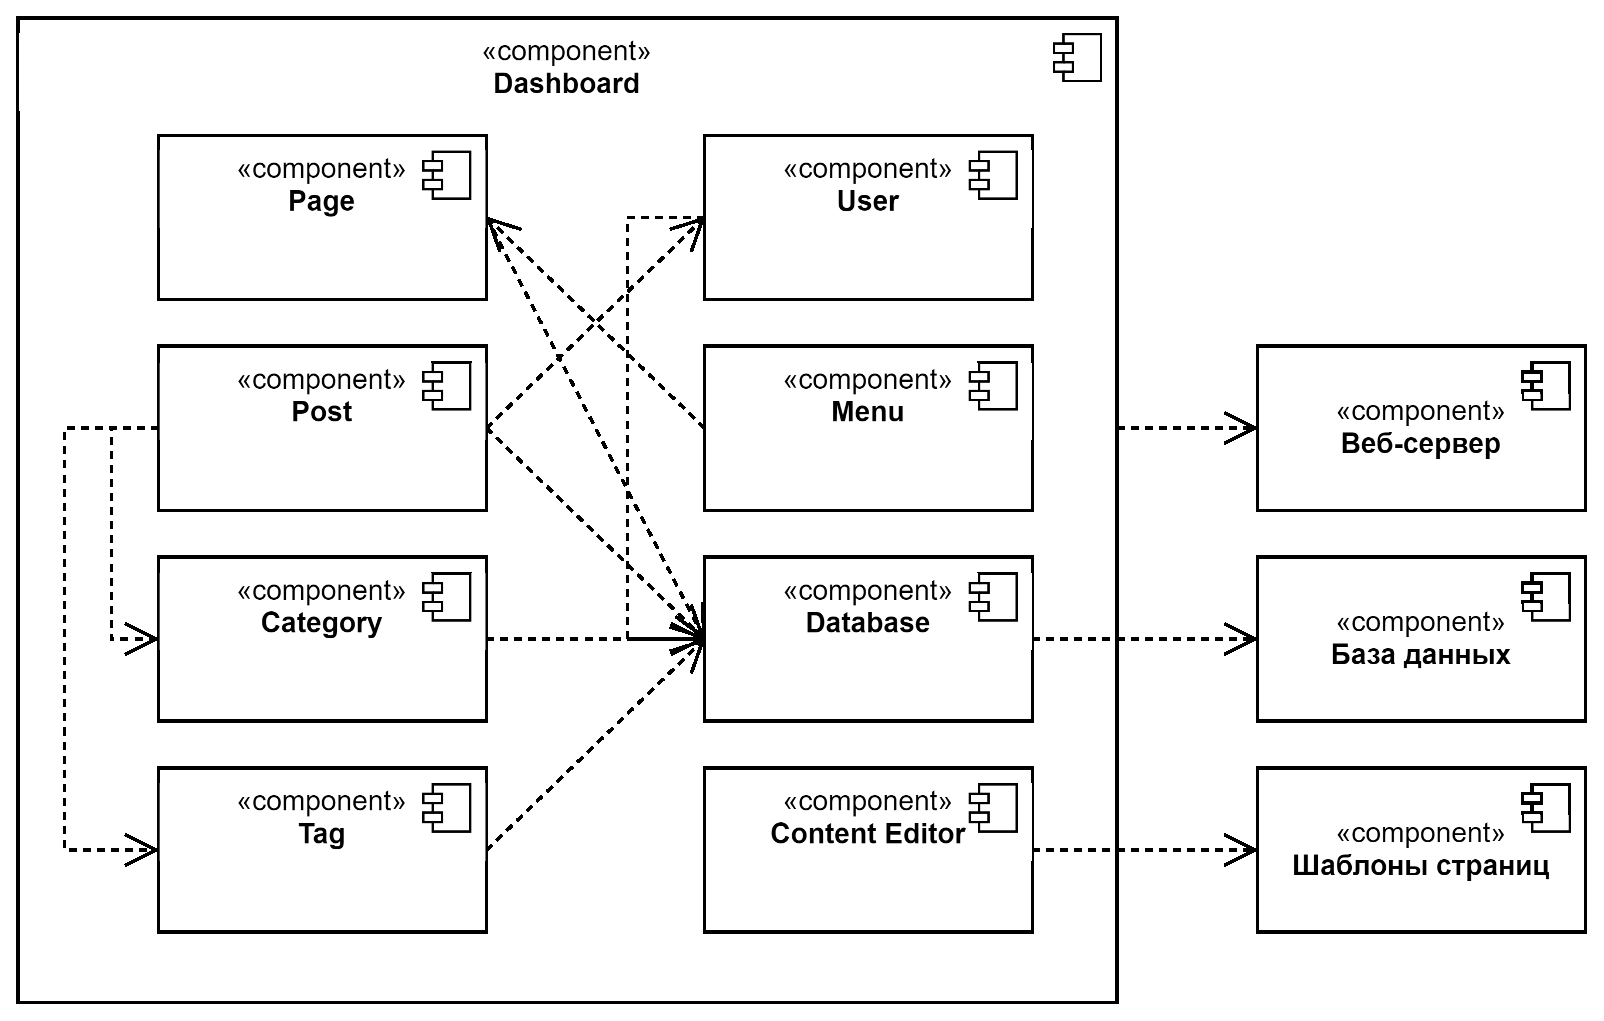
\includegraphics[width=1\linewidth]{comp}}
	\caption{Диаграмма компонентов}
	\label{comp:image}
\end{figure}

Описание компонентов программной системы:
\begin{enumerate}
	\item Page -- отвечает за создание и управление статическими страницами и организацию разделов сайта.
	\item Post -- используется для управления динамическим контентом, таким как статьи в блоге, новости, обновления и другие материалы, которые публикуются регулярно.
	\item Category -- используется для организации контента на сайте, содержит функции для структурирования постов по темам или разделам.
	\item Tag -- используется для дополнительной классификации контента, предоставляет более гибкую систему организации, чем категории, позволяя распределять посты по ключевым словам или темам.
	\item User -- этот компонент управляет информацией о пользователях сайта. Включает создание, редактирование и удаление учетных записей, управление ролями и правами доступа.
	\item Menu -- обеспечивает навигацию по сайту. Этот компонент позволяет создавать и управлять навигационными меню, которые могут содержать ссылки на страницы, посты, категории и другие элементы сайта.
	\item Content Editor -- представляет инструмент для создания и редактирования текстового и мультимедийного контента на сайте. Обычно он включает в себя визуальный интерфейс который позволяет пользователям форматировать текст, вставлять изображения, видео, ссылки и другие элементы без необходимости писать HTML код.
	\item Database -- обеспечивает создание и управление данными которые храняться в таблицах БД, отвечает за выполнение запросов к базе данных для получения, добавления, обновления и удаления информации.
\end{enumerate}

\subsubsection{Классы программной системы}
На рисунке \ref{ui1:image} представлена диаграмма классов программной системы.

\begin{figure}[ht]
	\center{
\includegraphics[width=1\linewidth]{class}}
	\caption{Диаграмма классов}
	\label{class:image}
\end{figure}

\subsection{Проектирование пользовательского интерфейса программной системы}

На основании требований к пользовательскому интерфейсу представленных в пункте \ref{interface_requirements} технического задания, был разработан интерфейс администранивной панели системы и интерфейс редактора контента. Для создания пользовательского интерфейса используется язык разметки HTML и веб-фреймворк Bootstrap 5.

На рисунке \ref{ui1:image} представлен макет главного окна однистративной панели CMS. Макет содержит следующие элементы:
\begin{enumerate}
	\item Навигационное меню для перехода в соответствующий раздел панели управления.
	\item Область отображения содержимого текущего раздела.
\end{enumerate}
\begin{figure}[ht]
	\center{\includegraphics[width=1\linewidth]{ui1}}
	\caption{Макет главного окна панели управления}
	\label{ui1:image}
\end{figure}
На рисунке \ref{ui2:image} представлен макет раздела управления страницами. Макет содержит следующие элементы:
\begin{enumerate}
	\item Кнопку "<Добавить страницу"> для добавленя новой страницы.
	\item Список страниц сайта.
	\item Название соответствующей страницы.
	\item Кнопки управления страницей.
\end{enumerate}
\begin{figure}[ht]
	\center{\includegraphics[width=1\linewidth]{ui2}}
	\caption{Макет раздела управления страницами}
	\label{ui2:image}
\end{figure}
На рисунке \ref{ui3:image} представлен макет раздела управления областями меню. Макет содержит следующие элементы:
\begin{enumerate}
	\item Список областей меню сайта.
	\item Кнопку "<Изменить"> для перехода на страницу управления пунктами выбранной области меню.
\end{enumerate}
\begin{figure}[ht]
	\center{\includegraphics[width=1\linewidth]{ui3}}
	\caption{Макет раздела управления областями меню}
	\label{ui3:image}
\end{figure}
На рисунке \ref{ui4:image} представлен макет раздела управления пунктами меню. Макет содержит следующие элементы:
\begin{enumerate}
	\item Кнопку "<Добавить"> для добавленя нового пункта меню.
	\item Список пунктов меню.
	\item Кнопку для просмотра дочерних пунктов меню.
\end{enumerate}
\begin{figure}[ht]
	\center{\includegraphics[width=1\linewidth]{ui4}}
	\caption{Макет раздела управления пунктами меню}
	\label{ui4:image}
\end{figure}